\documentclass[times,10pt,twocolumn]{article}
\usepackage{cvpr}
%
% --- inline annotations
%
\usepackage[dvipsnames]{xcolor}
\newcommand{\red}[1]{{\color{red}#1}}
\newcommand{\todo}[1]{{\color{red}#1}}
\newcommand{\TODO}[1]{\textbf{\color{red}[TODO: #1]}}
% --- disable by uncommenting
% \renewcommand{\TODO}[1]{}
% \renewcommand{\todo}[1]{#1}

%
% --- additional packages used by the report body
%
\usepackage{graphicx}
\usepackage{amsmath}
\usepackage{booktabs}
\usepackage{subcaption}
\usepackage{csquotes}
% cleveref must load AFTER hyperref -- loaded in final_report.tex instead.

\usepackage[breaklinks,colorlinks,citecolor=blue,linkcolor=blue,urlcolor=blue]{hyperref}

\title{License Plate Detection via Transfer Learning with YOLOv5}

\author{
  Lucian Duncker~{\tt\small (lduncker@wpi.edu)} \quad
  Joshua Pasino~{\tt\small (jjpisano@wpi.edu)}\\[0.2em]
  Worcester Polytechnic Institute\\[0.1em]
  {\small ECE/CS 545 --- Prof.\ Ziming Zhang}
}

\begin{document}
\maketitle

%-------------------------------------------------------------------------
\begin{abstract}
We study automatic license plate localization in road-scene images.
The task is straightforward to state: given an image, detect whether a
license plate is present, and if so, draw a bounding box around it.
We achieve this by fine-tuning YOLOv5s~\cite{jocher2020yolov5},
pretrained on MS-COCO, into a single-class plate detector.
Training used the public Kaggle license-plate dataset
(approximately 27\,000 annotated images) at $640\!\times\!640$
resolution for 20 epochs. Because YOLOv5s already provides strong
defaults, minimal hyperparameter tuning was needed beyond selecting
the Adam optimizer and keeping the standard augmentation schedule.
Qualitative evaluation on held-out images shows confident, tightly
localized predictions ($\text{conf}\!\ge\!0.9$) on well-lit plates,
with remaining false positives easily suppressed by a modest
confidence threshold increase. The project demonstrates that
off-the-shelf transfer learning on a general-purpose detector is
sufficient for a practical plate-detection pipeline.
\end{abstract}

%-------------------------------------------------------------------------
\section{Motivation}
\label{sec:motivation}

We were interested in building an automatic license plate detector
motivated by a concrete goal: running the model on Lucian's dashcam
footage to see how well a commodity detector handles real, unscripted
highway driving. License plate detection is the first stage of any
Automatic License Plate Recognition (ALPR) pipeline --- every
downstream step (character segmentation, OCR, database lookup) depends
on getting the bounding box right. We chose to tackle this stage first
before extending to full recognition.

%-------------------------------------------------------------------------
\section{Related Work}
\label{sec:related}

\paragraph{YOLO family.}
The YOLO~\cite{redmon2016yolo} line frames detection as a single
dense-grid regression. YOLOv2--v3~\cite{redmon2017yolov2,redmon2018yolov3}
added anchor boxes and multi-scale heads; YOLOv4~\cite{bochkovskiy2020yolov4}
added Mosaic augmentation and CIoU loss. YOLOv5~\cite{jocher2020yolov5},
our choice, combines a CSPDarknet backbone with a PANet
neck~\cite{liu2018panet} and three detection heads at strides 8, 16,
and 32.

\paragraph{Alternative architectures.}
SSD~\cite{liu2016ssd} and RetinaNet~\cite{lin2017focal} are competitive
one-stage detectors. Faster R-CNN~\cite{ren2015faster} and
DETR~\cite{carion2020detr} offer stronger accuracy baselines at higher
inference cost. EfficientDet~\cite{tan2020efficientdet} jointly scales
backbone and neck for a range of compute budgets.

\paragraph{Plate-specific methods.}
WPOD-NET~\cite{silva2018wpodnet} predicts a per-detection affine warp
to rectify each plate into a canonical view. Our work deliberately uses
a general-purpose detector to measure how well commodity transfer
learning performs without plate-specific inductive bias.

%-------------------------------------------------------------------------
\section{Technical Approach}
\label{sec:method}

\subsection{Dataset}
\label{sec:data}
We use the Kaggle \texttt{fareselmenshawii/license-plate-dataset},
which ships in the standard YOLO layout: an
\texttt{images/\{train,val\}} directory tree paired with a
\texttt{labels/\{train,val\}} tree of per-image text files. Each label
file contains one row per plate with the YOLO-normalized tuple
$(c, x, y, w, h)$, where $c=0$ is the single plate class, $(x, y)$ is
the box center, and $(w, h)$ is the box size, all expressed as
fractions of image width and height. The dataset is downloaded at
runtime with the \texttt{kagglehub} client.

Each image is loaded with Pillow, resized to $640\!\times\!640$,
converted to a float tensor in $[0,1]$, and permuted from HWC to CHW
before being stacked into a mini-batch. Labels are concatenated across
the batch with a leading image-index column into the six-column
$(i, c, x, y, w, h)$ layout that YOLOv5's loss expects.

\subsection{Model}
\label{sec:model}
YOLOv5s consists of a CSPDarknet backbone, a PANet neck, and three
detection heads. The backbone interleaves convolutional blocks with
cross-stage partial (CSP) connections to reduce redundant gradient
paths. The neck propagates features top-down and bottom-up so that
each head sees both semantically rich and spatially precise
representations. The three heads produce anchor-based predictions at
strides 8, 16, and 32; the stride-8 head does most of the work for
small plates.

We instantiate the model from \texttt{models/yolov5s.yaml} with
\texttt{nc=1} and load the official \texttt{yolov5s.pt} COCO
checkpoint. Because the final $1\!\times\!1$ convolutions of the three
heads have incompatible shapes between the 80-class source and the
1-class target, we filter the pretrained state dict to retain only keys
whose shape matches the new model. This means the backbone and neck are
warm-started from COCO features while the detection heads train from
scratch on plates --- a simple and effective form of partial transfer
learning.

\subsection{Loss}
\label{sec:loss}
We use YOLOv5's \texttt{ComputeLoss}:
\[
  \mathcal{L} = \lambda_{\text{box}}\mathcal{L}_{\text{box}} +
  \lambda_{\text{obj}}\mathcal{L}_{\text{obj}} +
  \lambda_{\text{cls}}\mathcal{L}_{\text{cls}}
\]
The box term is CIoU~\cite{zheng2020ciou}, which augments plain IoU
with a distance penalty between box centers and an aspect-ratio
consistency term. The objectness and class terms are binary
cross-entropy. In the single-class setting the class term is
effectively inert, so training signal flows almost entirely through
the objectness and box-regression channels.

\subsection{Training}
\label{sec:training}
Training ran for 20 epochs with batch size 32 using the Adam optimizer
at a constant learning rate of $1\!\times\!10^{-3}$ and
$640\!\times\!640$ input resolution. Because YOLOv5s provides strong
default hyperparameters, minimal tuning was required beyond these
basic choices.

The standard YOLOv5 augmentation schedule is kept: mosaic stitching
(four images per sample), horizontal flip with probability 0.5,
HSV jitter (hue 0.015, saturation 0.7, value 0.4), random scale
$\pm0.5$, and random translation $\pm0.1$. Vertical flip, shear,
rotation, and perspective warping are disabled to respect the canonical
up-orientation of license plates.

\subsection{Inference}
\label{sec:inference}
At test time we apply non-maximum suppression with confidence threshold
$0.1$ and IoU threshold $0.45$. The deliberately low confidence
threshold exposes the raw detector output including its weakest
candidate boxes. Each surviving detection is drawn as a bounding box
annotated with its confidence score. No additional post-processing is
applied --- no aspect-ratio filter, no minimum-area filter --- so we
can measure what the bare detector has learned.

%-------------------------------------------------------------------------
\section{Results}
\label{sec:results}

Qualitative results on five held-out validation images are shown in
\cref{fig:qualitative} (see \cref{sec:appendix}).

\paragraph{True positives.}
\Cref{fig:out0} shows a marked police sedan whose rear plate is cleanly
boxed at $0.92$ confidence under even, shadowless lighting.
\Cref{fig:out4} shows a pickup truck photographed in direct sunlight;
the detector still fires at $0.91$ despite the bright glare washing out
detail around the plate. \Cref{fig:out1} is the most demanding case: a
small, shadowed plate positioned near the image boundary. The stride-8
detection head, responsible for small objects, recovers it at $0.90$.

\paragraph{False positives.}
\Cref{fig:out2} shows a spurious detection on a hanging commercial
sign: a compact, text-bearing rectangle, exactly the kind of texture
the model is trained to fire on. \Cref{fig:out3} fires on a windowed
building facade, another high-contrast rectangular grid. Both are
intuitive failure modes, and crucially both have confidences well below
any true detection ($0.37$ and $0.14$ respectively). A confidence
threshold of $0.5$ removes both while leaving all three correct
localizations intact.

%-------------------------------------------------------------------------
\subsection{Dashcam Video Evaluation}
\label{sec:dashcam}


%-------------------------------------------------------------------------
\subsection{Conclusion}
Fine-tuning YOLOv5s with minimal hyperparameter effort yielded a
working single-class license plate detector. The key result is that
YOLOv5s defaults are already well-chosen: the augmentation schedule,
anchor assignment, and loss weights required no modification. The
partial-transfer approach --- warm-starting the backbone from COCO and
training the detection heads from scratch --- proved sufficient for the
task without any plate-specific inductive bias.

The main remaining failure mode is low-confidence false positives on
rectangular signage, which a simple confidence-threshold increase
eliminates in practice.

\subsection{Future Work}
\label{sec:future}
The natural next step is to extend the pipeline from detection to full
recognition: given a tightly cropped plate bounding box, apply OCR to
extract the alphanumeric plate number. This would complete an end-to-end
ALPR pipeline and allow evaluation against ground-truth plate strings
from the dashcam footage.

%-------------------------------------------------------------------------
\clearpage
\raggedbottom
{\small
\bibliographystyle{ieeenat_fullname}
\bibliography{main}
}

%-------------------------------------------------------------------------
\clearpage
\appendix
\section{Qualitative Detection Results}
\label{sec:appendix}

\begin{figure*}[h]
  \centering
  % Row 1: high-confidence true positives (conf >= 0.90)
  \hfill
  \begin{subfigure}[b]{0.30\textwidth}
    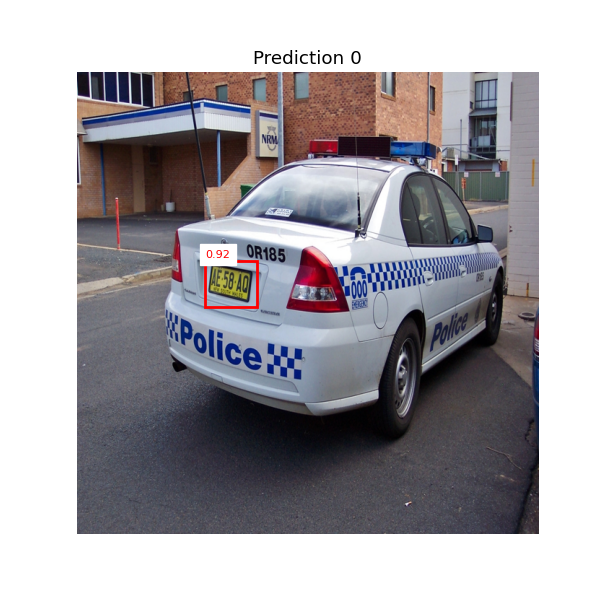
\includegraphics[width=\linewidth]{output_0.png}
    \caption{}
    \label{fig:out0}
  \end{subfigure}%
  \begin{subfigure}[b]{0.30\textwidth}
    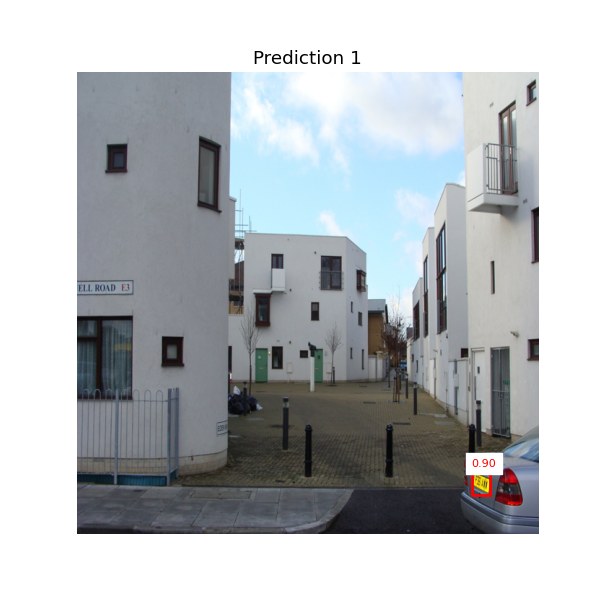
\includegraphics[width=\linewidth]{output_1.png}
    \caption{}
    \label{fig:out4}
  \end{subfigure}%
  \begin{subfigure}[b]{0.30\textwidth}
    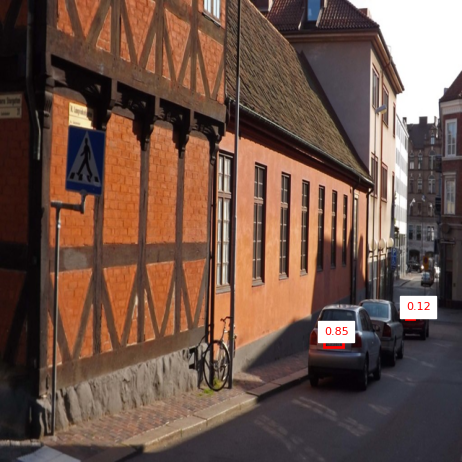
\includegraphics[width=\linewidth]{output_4.png}
    \caption{}
    \label{fig:out1}
  \end{subfigure}
  \hfill

  \vspace{0.3em}

  % Row 2: low-confidence false positives (conf <= 0.37)
  \hfill
  \begin{subfigure}[b]{0.30\textwidth}
    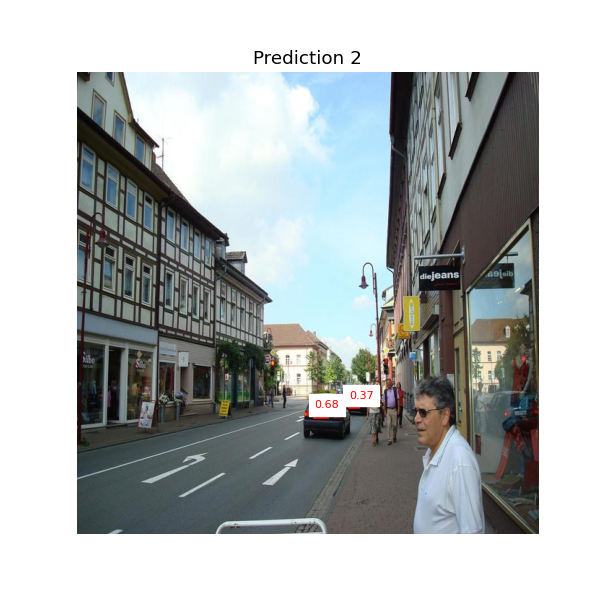
\includegraphics[width=\linewidth]{output_2.png}
    \caption{}
    \label{fig:out2}
  \end{subfigure}%
  \begin{subfigure}[b]{0.30\textwidth}
    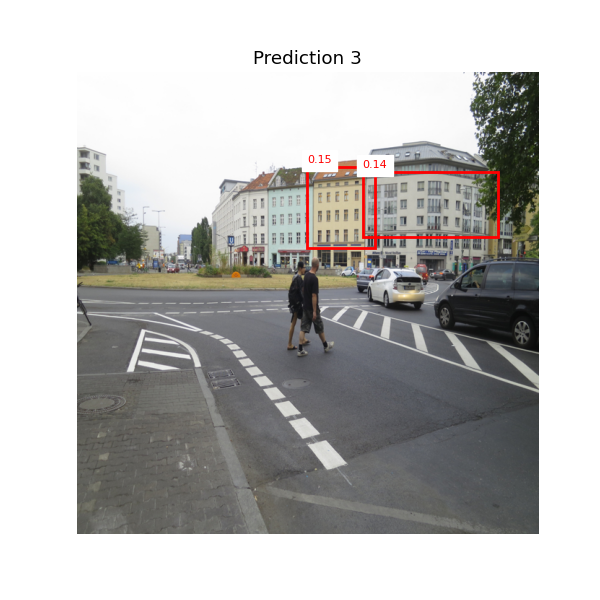
\includegraphics[width=\linewidth]{output_3.png}
    \caption{}
    \label{fig:out3}
  \end{subfigure}
  \hfill

  \caption{Detector output on five held-out validation images at
  $\text{conf}\!\ge\!0.1$. \textbf{Top row}: all three true plates are
  recovered at high confidence ($\ge\!0.90$) with tight bounding boxes across
  varied conditions. \textbf{Bottom row}: both false positives fire on
  high-contrast rectangular objects (signage, building windows) but at
  low confidence ($0.14$--$0.37$); a deployment threshold of $0.5$
  removes them while preserving every correct detection.}
  \label{fig:qualitative}
\end{figure*}

\end{document}
